%导言区
\documentclass[UTF8]{article}%设置了文档的类型为article,适用于撰写短篇文章或论文,并指定了UTF8中文字体
%引入宏包
\usepackage{ctex}       %中文支持
\usepackage{setspace}   %空白设置
\usepackage{abstract}   %摘要环境
\usepackage{amsmath}    %数学公式
\usepackage{graphicx}   %图像插入
\usepackage{booktabs}   %表格线条
\usepackage{array}      %列对齐
\usepackage{hyperref}   %超链接

%图片路径设置Figures/文件夹下
\graphicspath{{figures/}}       

%超链接显示样式设置
\hypersetup{colorlinks = true,                  % 颜色
    bookmarksopen = true,                       % 书签展开
    bookmarksnumbered = true,                   % 编号
    pdftitle = latex快速入门手册,                  %PDF标题
    pdfauthor =farfar}                          %PDF作者

%参考文献样式
\bibliographystyle{plain}% 参考文献引用格式
\newcommand{\upcite}[1]{\textsuperscript{\cite{#1}}} %定义一个新的命令\upcite,用于生成上标格式的引用

%目录格式
\renewcommand{\contentsname}{\centerline{Contents}} %目录标题居中

%文档标题、作者和日期
\title{\heiti\zihao{2} latex快速入门手册}      %设置标题,使用\heiti(黑体)和\zihao(字号)调整字体样式和大小
\author{\songti farfar}                     %设置了作者名称,songti(宋体)
\date{\today}                               %设置了日期,\today为当天日期,也可以设置为固定的时间

%正文区
\begin{document}

    \maketitle              %生成标题页
    \thispagestyle{empty}   %设置本页没有页眉和页脚

%摘要
\begin{abstract}            
    大家好,欢迎来到farfar的AI4S日记! 今天介绍如何快速使用Latex。
\end{abstract}

%目录
\tableofcontents

%章节和子章节
\section{Latex下载与安装}
本次教程应用的Latex编辑排版环境是TeX Live +Visual Studio Code,在官网上安装,并按照教程配置环境即可。

\section{Letex基础内容}
接下来,我们依次介绍如何插入公式和特殊符号、图片、表格以及参考文献。

\subsection{公式和特殊符号}
数学公式不用记忆,在线网址\url{https://www.latexlive.com/}轻松解决 
\[ x^{2 \alpha} - 1 = y_{ij} + y_{ij}  \]
\[ \int\limits_0^1 x^2 + y^2 \ dx \]
\[ \sum_{i=1}^{\infty} \frac{1}{n^s} = \prod_p \frac{1}{1 - p^{-s}} \]
\[\mathcal{B} = \{B_{\alpha} \in \mathcal{T}\, |\,  U = \bigcup B_{\alpha} \forall U \in \mathcal{T} \}\]

引用公式1 \ref{eq:vsphere}
   \begin{equation} %公式
     \label{eq:vsphere}
       V = \frac{4}{3}\pi r^3
       \end{equation}

\subsection{图片}
图\ref{Fig:1}是farfar头像
\begin{figure}[!h]                                  %使用figure环境插入图片,!h参数使其在当前位置显示
    \centering                                      %居中显示
    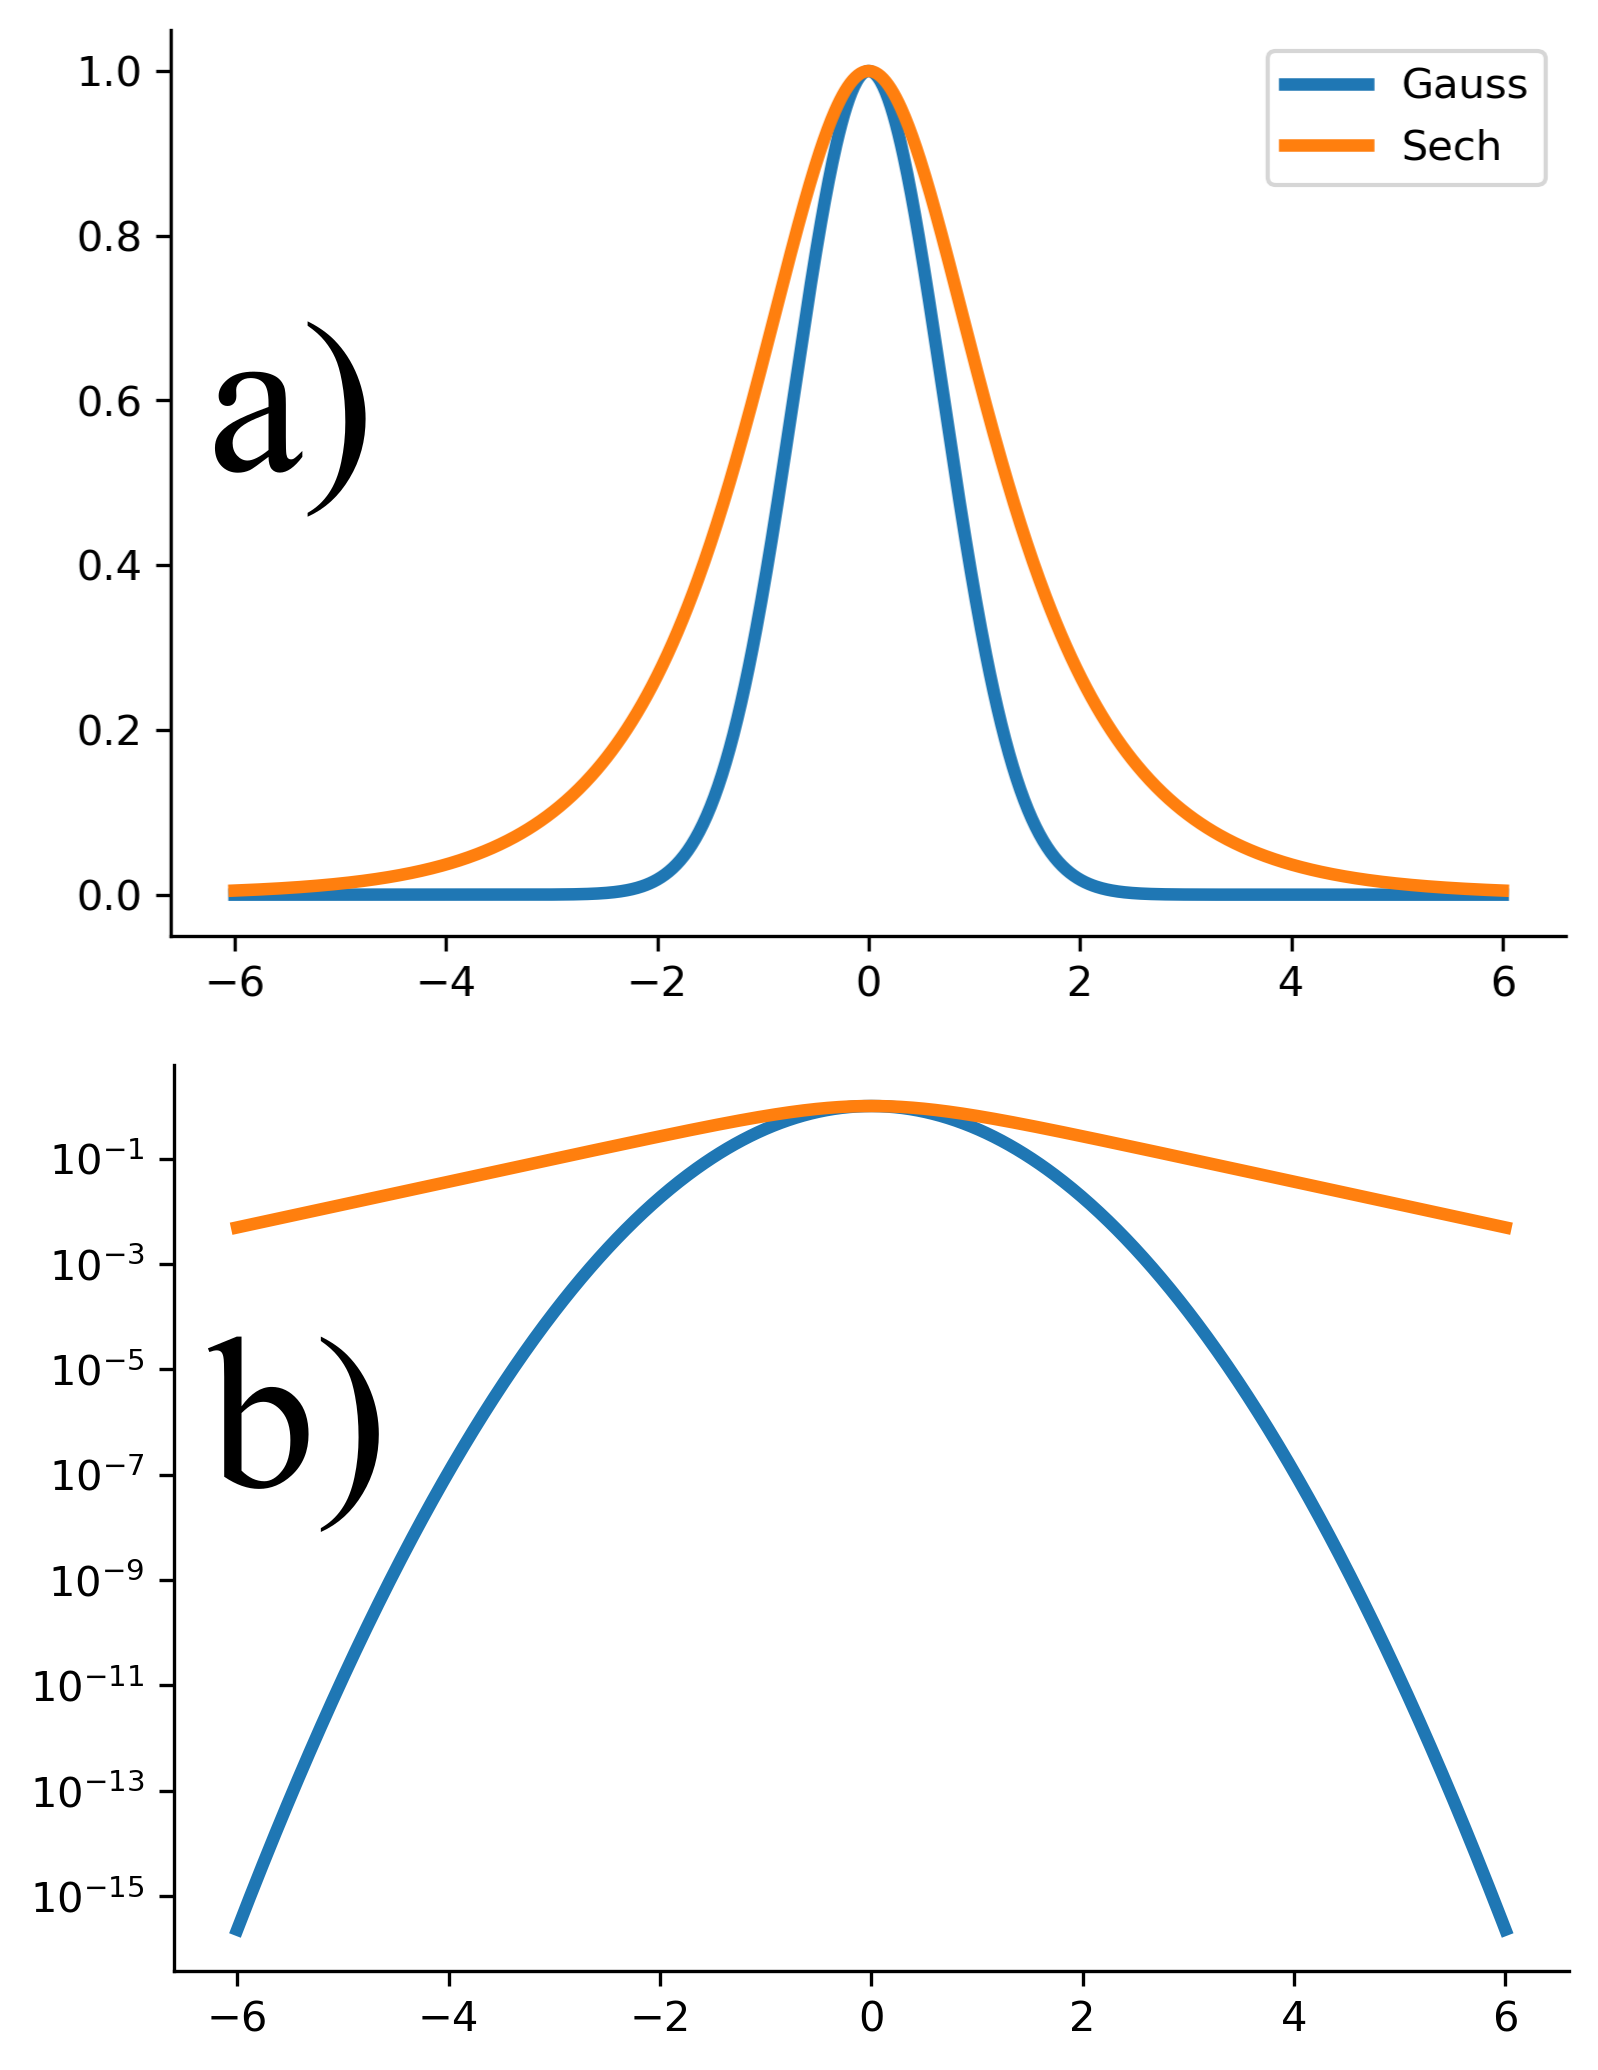
\includegraphics[scale=0.2]{farfar.png}        %插入图片文件farfar.jpeg,并将图片的尺寸缩放到原始大小的20%
    \caption{this is farfar}                        %为图片提供标题
    \label{Fig:1}                                   %为图片分配一个标签,可以引用
\end{figure}

\subsection{表格}
在线网址轻松生成\url{https://www.tablesgenerator.com
/latex_tables}
表格\ref{table:1}是第一个表格
\begin{table}[h!]                                   %使用table环境创建表格,并设置列格式和标题。
    \centering                                      %居中显示
    \begin{tabular}{|c|c c c||}                     %开始一个tabular环境,创建一个由四列组成的表格,列的对齐方式默认为居中(c),两侧的竖线表示列的边界
     \hline                                         %画一条水平线,通常是表格的顶部边框。
     C1 & C2 & C3 & C4 \\ [0.5ex]                   %定义表格的第一行,包含四列的标题,分别为C1、C2、C2和C3。\\表示一行结束,[0.5ex]在行末添加了额外的垂直间距。
     \hline\hline                                   %画两条连续的水平线
     1 & 6 & 87837 & 787 \\                         %定义表格的第二行,用&分隔对应的数据
     2 & 7 & 78 & 5415 \\
     3 & 545 & 778 & 7507 \\
     \hline
    \end{tabular}                                   %结束tabular环境
    \caption{This is a table.}                      %为表格添加标题
    \label{table:1}                                 %为表格分配一个标签,方便在文档中引用
    \end{table}

    
\subsection{参考文献}
引用文献一\cite{1}。 引用文献一\upcite{1}。%系统引用命令cite,自定义引用命令upcite

引用文献二\cite{2}。 引用文献二\upcite{2}。
\bibliography{ref}                       %文献引用文档ref.bib 

%文档结束
\end{document}